Commençons par raisonner géométriquement dans le cas où les six premiers points sont distincts, et le polygone $A_1 A_2 A_3 A_4 A_5 A_6$ convexe.
Nous avons alors une figure codée du type suivant où $M_i$ désigne le milieu du segment $[A_i A_{i+1}]$ 
\emph{(on prendra garde que l'on ne sait pas encore que $A_7 = A_1$ contrairement à ce que nous constatons sur le dessin)}.
Nous verrons ensuite comment passer au cas général car on peut avoir un polygone $A_1 A_2 A_3 A_4 A_5 A_6$ non convexe, ainsi que certains des points $A_i$ et $A_{i+1}$ égaux, voir tous, 

\vspace{1em}

\begin{center}
	\fbox{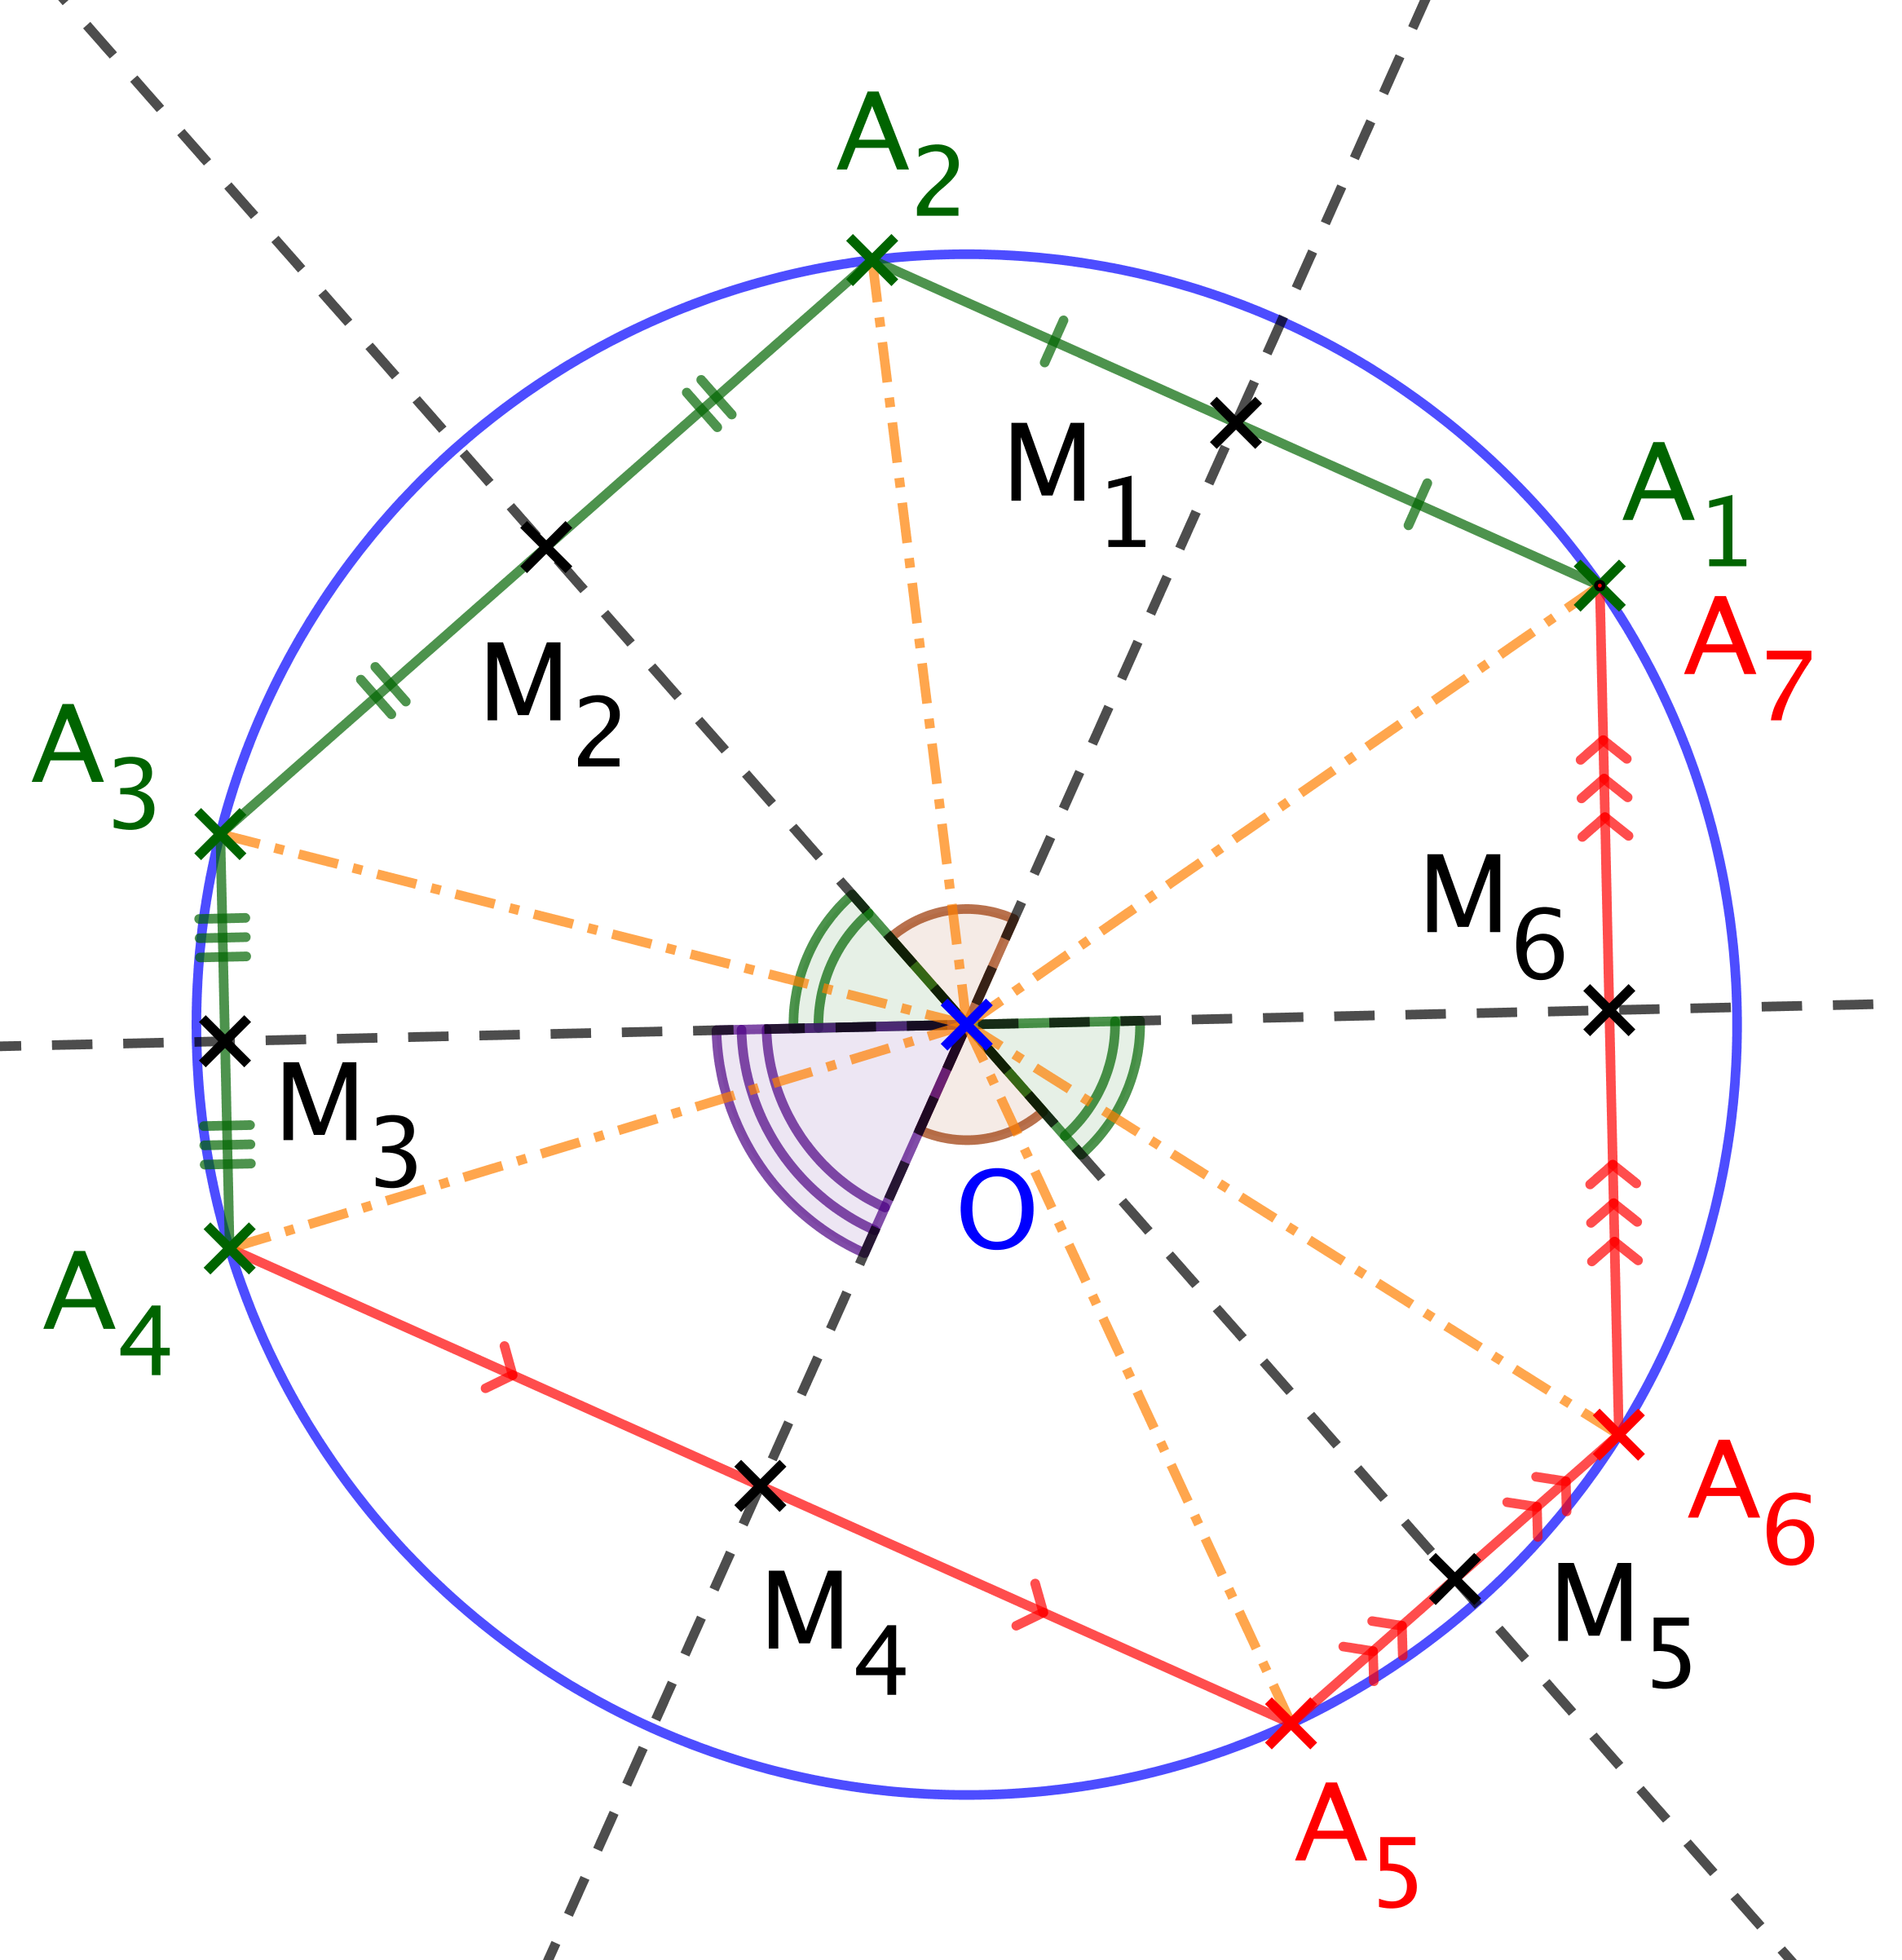
\includegraphics[scale = .6]{proof-1-Mi.png}}
\end{center}

\vspace{1em}


% ---------------- %


Pour $i \in \NNs$ , nous avons les faits suivants.
\begin{enumerate}
	\item $(OM_i)$ est une bissectrice du triangle $O A_i A_{i+1}$ .

	\item $(M_i M_{i+3}) = (O M_i) = (O M_{i+3})$ est la médiatrice commune aux segments parallèles $[A_i A_{i+1}]$ et $[A_{i+3} A_{i+4}]$ .

	\item $\vangleorient{OM_i}{OM_{i+1}} = \vangleorient{OM_{i+3}}{OM_{i+4}}$ car ce sont des angles opposés par le sommet grâce au fait précédent. Ceci justifie au passage les codages de la figure ci-dessus.
\end{enumerate}


\medskip


Notant $\alpha_i = \vangleorient{OA_i}{OM_i}$ , nous avons alors les nouveaux faits suivants.
\begin{enumerate}[start=4]
	\item $\alpha_i = \vangleorient{OM_i}{OA_{i+1}}$ d'après le fait 1.
	
	\item $\alpha_i + \alpha_{i+1} = \vangleorient{OM_i}{OM_{i+1}}$ d'après le fait précédent.
	
	\item $\alpha_i + \alpha_{i+1} = \alpha_{i+3} + \alpha_{i+4}$ d'après les faits 3 et 5.
\end{enumerate}


\medskip


La dernière identité nous donne en particulier les égalités suivantes.

\begin{itemize}[label=\small\textbullet]
	\item \textbf{[L1]} : 
	      $\alpha_1 + \alpha_{2} = \alpha_{4} + \alpha_{5}$

	\item \textbf{[L2]} : 
	      $\alpha_2 + \alpha_{3} = \alpha_{5} + \alpha_{6}$

	\item \textbf{[L3]} : 
	      $\alpha_3 + \alpha_{4} = \alpha_{6} + \alpha_{7}$
\end{itemize}


\medskip


\textbf{[L3] $-$ [L2] $+$ [L1]} aboutit à $\alpha_1 + \alpha_4 = \alpha_7 + \alpha_4$ d'où $\alpha_1 = \alpha_7$ . On y est presque même si cette égalité seule ne suffit pas à conclure.


\medskip


Notons ensuite $\Pi$ l'angle plat
\footnote{
	Ne pas confondre $\Pi$ qui est un objet géométrique avec $\pi$ l'une de ses mesures en radian.
},
de sorte que $2 \Pi \eq[def] \Pi + \Pi$ est l'angle nul qui sera noté $\Sigma_0$ .
Nous avons alors :

\vspace{-1em}

\begin{flalign*}
	\Sigma_0
		&= \vangleorient{OM_1}{OM_1}
		& \\
		&= \sum_{i=1}^{6} \vangleorient{OM_i}{OM_{i+1}}
		 +
		   \vangleorient{OM_7}{OM_1}
		& \\
		&= \sum_{i=1}^{3} \vangleorient{OM_i}{OM_{i+1}}
		 +
		   \sum_{i=1}^{3} \vangleorient{OM_{i+3}}{OM_{i+4}}
		 +
		   \vangleorient{OM_7}{OM_1}
		& \\
		&= 2 \sum_{i=1}^{3} \vangleorient{OM_i}{OM_{i+1}}
		 +
		   \vangleorient{OM_7}{OM_1}
		& \text{\small Voir le fait 3.} 
		& \\
		&= 2 \vangleorient{OM_1}{OM_4}
		 +
		   \vangleorient{OM_7}{OM_1}
		& \\
		&= 2 \Pi
		 +
		   \vangleorient{OM_7}{OM_1}
		& \text{\small Voir le fait 2.}
		& \\
		&= \vangleorient{OM_7}{OM_1}
		& \text{\small Car $2 \Pi = \Sigma_0$ .}
		& \\
\end{flalign*}

\vspace{-1em}


Ceci nous fournit ensuite :

\vspace{-1em}

\begin{flalign*}
	\vangleorient{OA_1}{OA_7}
		&= \vangleorient{OA_1}{OM_1}
		 + \vangleorient{OM_1}{OM_7}
		 + \vangleorient{OM_7}{OA_7}
		& \\
		&= \alpha_1
		 - \Sigma_0
		 - \alpha_7
		& \\
		&= \Sigma_0
		& \text{\small Car $\alpha_1 = \alpha_7$ .}
		& \\
\end{flalign*}

\vspace{-1em}

Finalement $\vect{OA_1}$ et $\vect{OA_7}$ sont colinéaires et de même sens ce qui implique que $A_7 = A_1$ \emph{(pourquoi ?)}. Ouf !
Il nous reste à passer de notre cas très particulier au cas général avec sa myriade d'exceptions.
Ce passage se fait via les constatations suivantes.
\begin{enumerate}
	\item La propriété de convexité n'est à aucun moment utilisé dans les calculs d'angles orientés.
	Elle a juste permis de construire un dessin sur lequel poser sa réflexion.

	\item Plus gênante a priori est la possibilité d'avoir $A_{i+1} = A_i$ .
	Le lecteur vérifiera sans peine qu'il suffit dans ce cas de poser $M_i \eq[def] A_i$ pour que les calculs restent valables.
\end{enumerate}
